\documentclass[../ClassicThesis.tex]{subfiles}
\begin{document}

%************************************************
\chapter{Plates}\label{ch:plates}
%************************************************

\section{Plates Can Be Found Inherently, by Extruding or by Stacking}

There are multiple approaches for finding plates contained in a 3D~mesh. Two of these concepts, inherent plates \cite[p.~32]{master-thesis} and extrusion \cite[p.~28]{master-thesis}, are based on existing algorithms. The third approach, stacking plates, was built from the ground up.

Inherent plates are modeled in the mesh, with both a top and a bottom side (see Figure~\ref{fig:inhplates}). Between these, a plate is constructed. This is the most obvious approach, since it finds plates which a human would identify as well. It is discussed in Section~\sectionref{sec:inherentplates}. The second approach, extruding plates, uses the mesh surface to extrude plates into the object (Figure~\ref{fig:extplates}). It is inspired by the extrusion manufacturing process, where a malleable material is pressed through a die. Here, a flat part of the model's surface is translated along its normal, resulting in the opposite side of the plate. This is described further in Section~\sectionref{sec:extrudedplates}. Our algorithm uses a combination of these two concepts. First, the model is searched for inherent plates. Afterwards, all surfaces of the model which were not used for creating a plate yet are forwarded to the extruding algorithm. While the first step finds plates which were actually sculpted in the model, the second step approximates a filled objects hull. Thus, we can handle complex meshes which feature both types of plates. 

The concept of stacking plates is described in Section~\sectionref{sec:stackedplates}. The model is sliced in regular intervals, with plates being created based on the cross sections. When these plates are put on top of each other, they approximate the original model (Figure~\ref{fig:staplates}). Additionally, special plates, called shafts, are added. These are perpendicular to the other plates and help with aligning them during assembly.

\begin{figure}
    \centering
    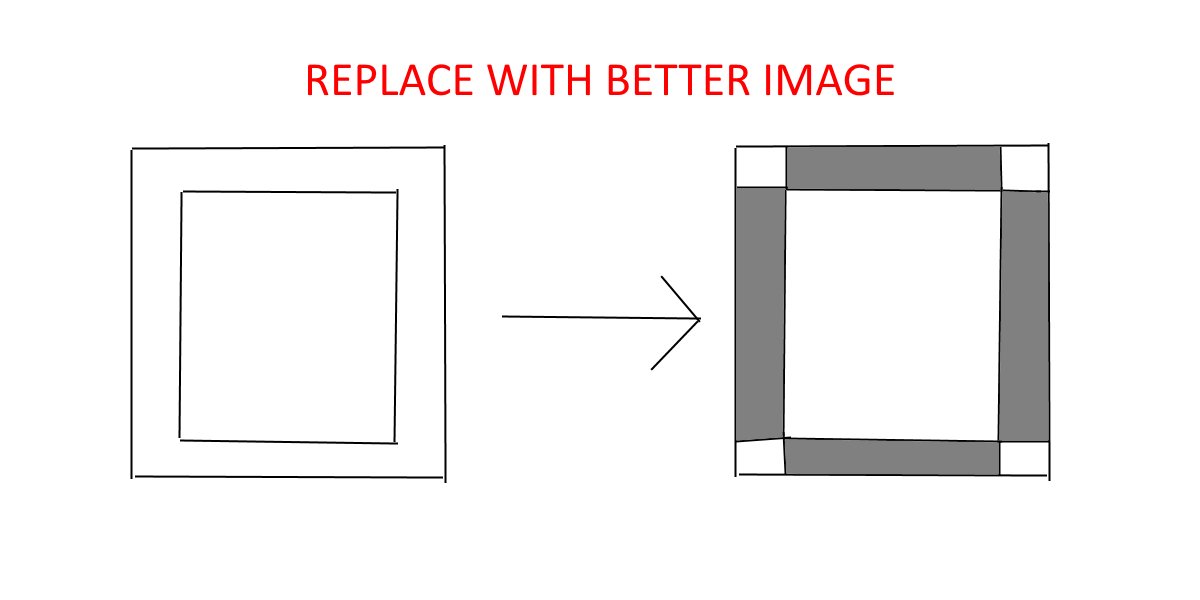
\includegraphics[width=1.0\columnwidth]{Images/plates_inherentplates.png}
    \caption{Finding inherent plates.}
    \label{fig:inhplates}
\end{figure}

\begin{figure}
    \centering
    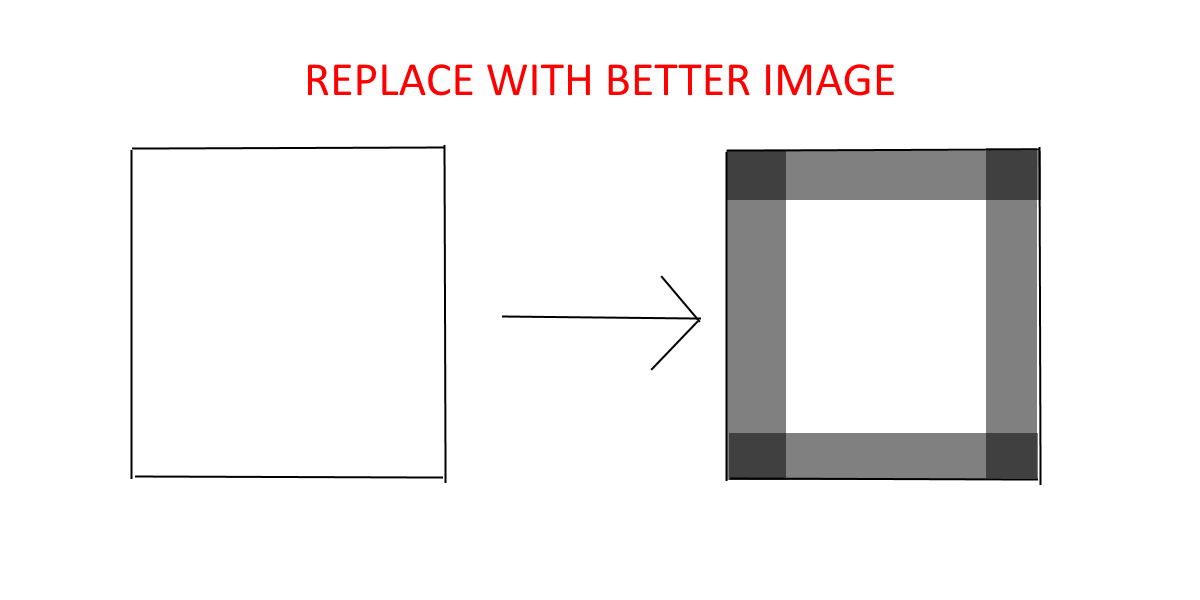
\includegraphics[width=1.0\columnwidth]{Images/plates_extrudedplates.png}
    \caption{Finding extruded plates.}
    \label{fig:extplates}
\end{figure}

\begin{figure}
    \centering
    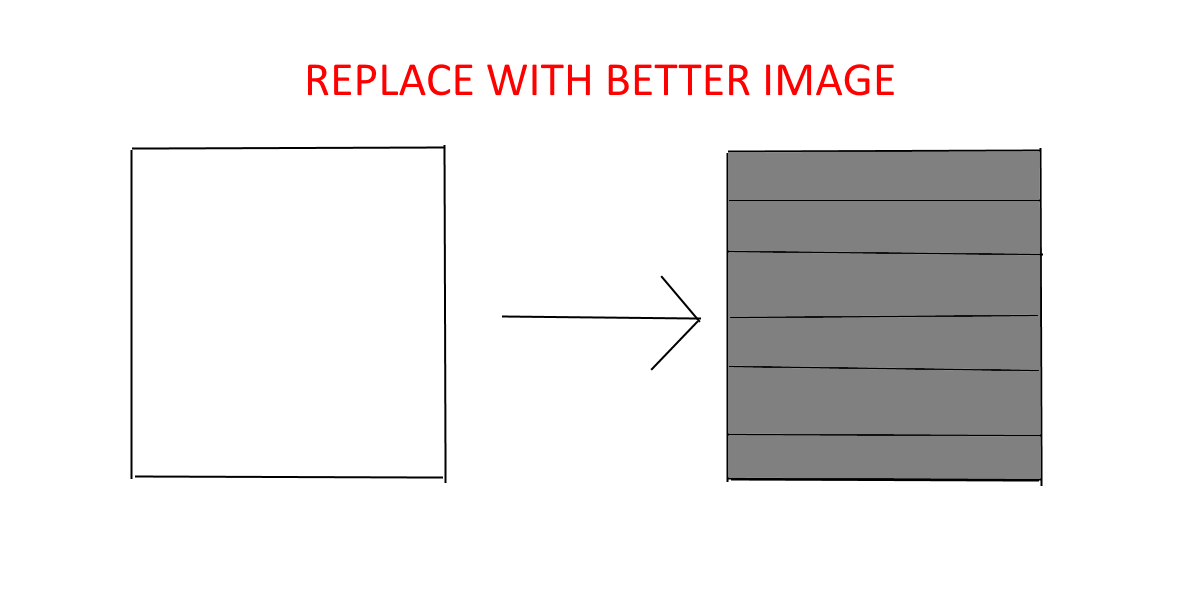
\includegraphics[width=1.0\columnwidth]{Images/plates_stackedplates.png}
    \caption{Finding stacked plates.}
    \label{fig:staplates}
\end{figure}

\section{Plates Are Generated from Planar Shapes}

Before these plate finding algorithms can process the model, it has to be prepared properly. The surface has to analyzed, with the faces being grouped into planar shapes. These shapes can be used as surfaces of plates. 

{\platener} solves this by running multiple pipeline steps beforehand. The first, called \emph{CoplanarFaces}, recreates planar shapes which have been divided when the model was triangulated by the creator. It groups the model's faces based on two test: The faces have to be connected and the angle between their normals must not exceed a given threshold. This step is described in Section~\sectionref{sub:coplanarfaces}. In the next step, \emph{edgeLoops} are created based on the previously generated groups of faces. An \emph{edgeLoop} is a list of vertices, describing a shape which consists of multiple faces. Only the outer edges of the shape are stored, since the triangulation of the mesh is not relevant for \platener{}. These \emph{edgeLoops} are created by the \emph{ShapesFinder}, which is discussed in Section~\sectionref{sub:shapesfinder}. The \emph{ShapesFinder} can create multiple \emph{edgeLoops} for one shape. This means that the shape contains holes. In order to differentiate between the shapes and the contour, another pipeline step is run, which is called \emph{HoleDetection}. It separates these by calculating the \emph{edgeLoops'} area. This is further explained in Section~\sectionref{sub:holedetection}.

The result of these calculations is a list of shapes, which contain one or multiple \emph{edgeLoops}. A label contains information about whether the \emph{edgeLoop} is the shapes contour or a hole.

\subsection{Coplanar Faces Are Grouped Based on Their Normal}\label{sub:coplanarfaces}

\begin{figure}
    \centering
    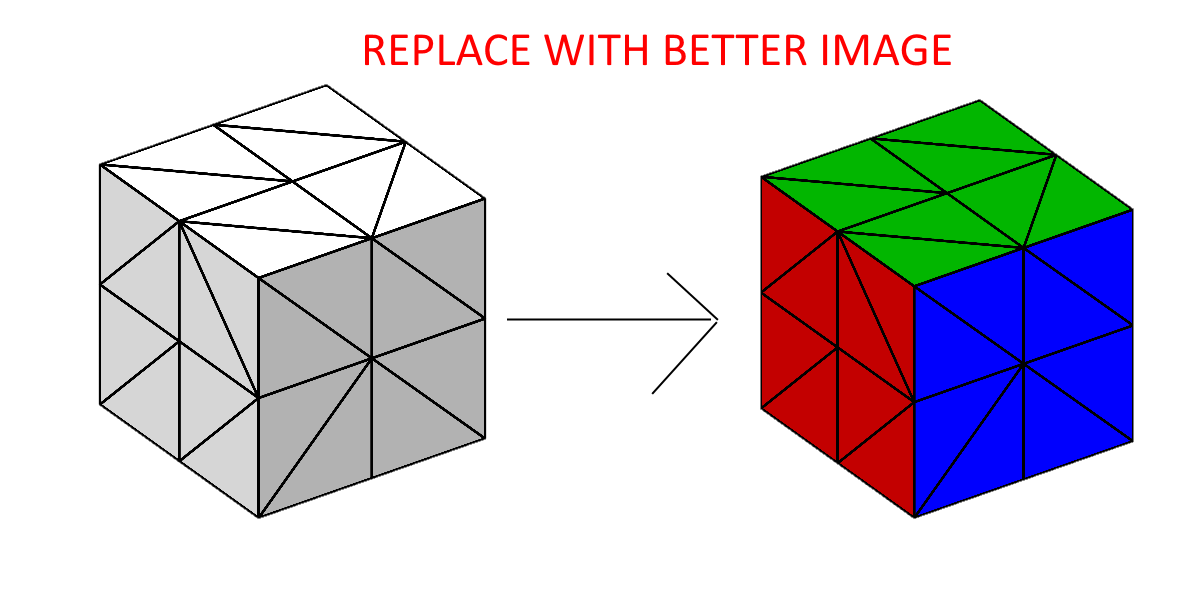
\includegraphics[width=1.0\columnwidth]{Images/plates_coplanar.png}
    \caption{Finding inherent surfaces.}
    \label{fig:coplanar}
\end{figure}

By definition, faces are called coplanar if they lie in the same plane. For our purposes, we extend this by the requirement that the face have to be directly connected as well. This allows grouping them into planar shapes. The algorithm for finding coplanar faces requires the models to be stored as a face-vertex mesh. This is calculated by {\meshlib}, the library used for importing models. In a face-vertex mesh, each vertex and each face is assigned an index. Three lookup tables are created: These contain the faces, vertices and face normals of the mesh separately. Figure~\ref{fig:facevertexmesh} shows an annotated mesh and the resulting lookup tables. The face lookup table contains the face indices and the indices of the vertices which compose the faces. Searching these in the vertex lookup table yields the coordinates of the vertices. The entries in the normal lookup table correspond with those in the face lookup table. For example, the normal of the face with the index~1 is located at index~1 in the normal lookup table. Face-vertex meshes enable faster adjacency checks than normal meshes, since vertex equality checks can be done by comparing the vertex indices. In fact, the \emph{CoplanarFaces} step's computation time was reduced from 736~ms to 18~ms when processing a mesh with 2400 faces\footnote{This was measured on a Intel{\textregistered}~Core{\texttrademark}~i5-2400~CPU with 8~GB of RAM, running Windows~8.1~Pro and Node v0.12.7.} by using a face-vertex mesh based implementation.

\begin{figure}
  \centering
  \begin{subfigure}[t]{0.8\textwidth}
    \centering
    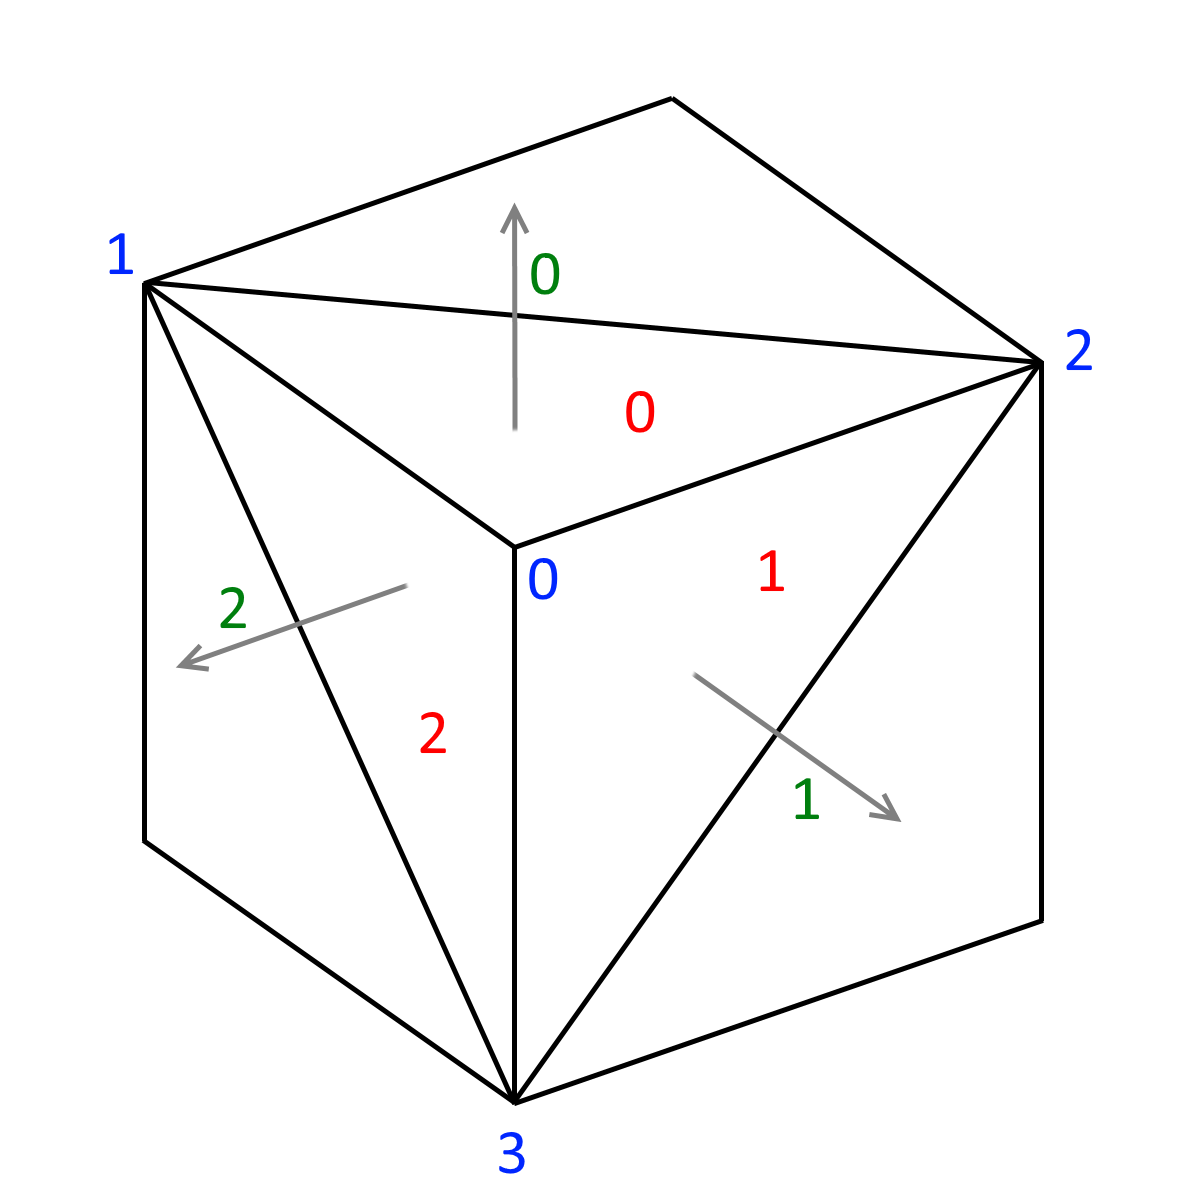
\includegraphics[width=0.8\textwidth]{Images/facevertexmesh.png}
    \caption{Partly annotated mesh. Face are marked in red, vertices in blue and normals in green.}
    \vspace{.5cm}
  \end{subfigure}
  \begin{subfigure}[t]{0.32\textwidth}
    \centering
    \begin{tabular}{ | l | l | }
      \hline
      index & vertices \\ \hline
      0 & 0, 1, 2 \\ \hline
      1 & 0, 2, 3 \\ \hline
      2 & 0, 3, 1 \\ \hline
      ... & ... \\
      \hline
    \end{tabular}
    \caption{Face lookup table.}
  \end{subfigure}
  \begin{subfigure}[t]{0.32\textwidth}
    \centering
    \begin{tabular}{ | l | l | }
      \hline
      index & coordinates \\ \hline
      0 & (1, 1, 1) \\ \hline
      1 & (0, 1, 1) \\ \hline
      2 & (1, 0, 1) \\ \hline
      3 & (1, 1, 0) \\ \hline
      ... & ... \\
      \hline
    \end{tabular}
    \caption{Vertex lookup table.}
  \end{subfigure}
  \begin{subfigure}[t]{0.32\textwidth}
    \centering
    \begin{tabular}{ | l | l | }
      \hline
      index & direction \\ \hline
      0 & (0, 0, 1) \\ \hline
      1 & (1, 0, 0) \\ \hline
      2 & (0, 1, 0) \\ \hline
      ... & ... \\
      \hline
    \end{tabular}
    \caption{Normal lookup table.}
  \end{subfigure}
  \caption{Example lookup tables of a face-vertex mesh.}
  \label{fig:facevertexmesh}
\end{figure}

In order to enable further computations, two more lookup tables are added: One contains all edges belonging to each face, while the second one allows looking up the faces adjacent to an edge. The edges are stored as a sorted pair of vertex indices. In the face-vertex mesh shown in Figure~\ref{fig:facevertexmesh} the face with the index~1 consists of the edges (0,~2), (0,~3) and (2,~3). Correspondingly, the edge (0,~2) refers to the faces~0 and~1. Both lists can be created in one single pass (see Listing~\ref{lst:lookuptables}).

\begin{listing}
\begin{minted}[
linenos
]{coffeescript}
setupFaceEdgeEdgeFaceLookup: ->
  for faceIndex in [0...faceCount]
    # Avoid double edges by sorting vertices
    { min_vertex
      mid_vertex
      max_vertex } = @findMinMidMaxVertex()
    # Register which edges this triangle uses.
    @addEntryToEdgeFaceMap(min_vertex, mid_vertex, faceIndex)
    @addEntryToEdgeFaceMap(mid_vertex, max_vertex, faceIndex)
    @addEntryToEdgeFaceMap(min_vertex, max_vertex, faceIndex)
    # Set the edges that make up this triangle.
    @faceVertexMesh.faceToEdges[faceIndex] = [
      [min_vertex, mid_vertex]
      [mid_vertex, max_vertex]
      [min_vertex, max_vertex]
    ]
\end{minted}
\caption{Simplified lookup table generation.}
\label{lst:lookuptables}
\end{listing}

Using these lookup tables, the faces are grouped. A face group contains faces which are connected and are coplanar. This in done by iterating over all faces. When a face is found which has not been visited yet, a new face group is started. Now all of the face's edges are pushed to a queue, along with the current face index. Afterwards, we start working on the queue, using a breadth-first approach. The processing function is shown in Listing~\ref{lst:traverseadjacent}.

\begin{listing}
\begin{minted}[
linenos,breaklines
]{coffeescript}
traverseAdjacentFaces: (...) ->
  if edgeQueue.length is 0
    return
  { edge, faceIndex } = edgeQueue.shift()
    faceNormal = @faceVertexMesh.getFaceNormal(faceIndex)
  # get the faces from the edge
  adjacentFaces = @faceVertexMesh.getFacesFromEdge(
    edge[0]
    edge[1]
  )
  continued = false
  for nextFaceIndex in adjacentFaces when nextFaceIndex isnt faceIndex
    # check if faces are coplanar
    # [...]
\end{minted}
\caption{Function repeated for each edge in queue.}
\label{lst:traverseadjacent}
\end{listing}

This is implemented as a \emph{tail recursion}. First, the length of the queue is checked. If there a no more edges waiting to be processed, we can jump out of the recursion and continue searching for new groups. Otherwise, we first get the normal of the face from which we came. Next, we extract the new face from the edge and get the face's normal as well. After checking the faces' coplanarity, we signal that there may be more elements in the queue by calling \mintinline{coffeescript}{recur}.

Listing \ref{lst:coplanarcheck} shows the coplanarity check. \mintinline{coffeescript}{isAngleZero} calculates the angle between the normals and compares it to zero. This is done even if the new face was already visited. If the faces are not coplanar, the edge is added to the group's outer edges. This list is used in the \emph{ShapesFinder} when merging the faces to one shape. In case of coplanarity, we now check if the face was visited. If it was not, it is added to the face group. Additionally, an entry is added to the \mintinline{coffeescript}{faceToFaceGroup} lookup table and the face is marked as visited. After fetching the face's edges, they are pushed into the queue. The algorithm is visualized in Figure~\ref{fig:coplanar_algorithm}.

\begin{listing}
\begin{minted}[
linenos,breaklines
]{coffeescript}
if @isAngleZero(faceNormal, nextFaceNormal)
  if not faceVisited[nextFaceIndex]
    faceGroup.push(nextFaceIndex)
    groupNormal.add(nextFaceNormal)
    @faceToFaceGroup[nextFaceIndex] = faceGroupIndex
    faceVisited[nextFaceIndex] = true
    adjacentEdges = @faceVertexMesh.getEdgesFromFace(nextFaceIndex)
    for nextEdge in adjacentEdges when not Util.arrayEquals edge, nextEdge
      edgeQueue.push({ edge: nextEdge, faceIndex: nextFaceIndex })
else
  outerEdgeGroup.push(edge)
\end{minted}
\caption{Check for coplanar faces.}
\label{lst:coplanarcheck}
\end{listing}

\begin{figure}
  \centering
  \begin{subfigure}[t]{0.4\textwidth}
    \centering
    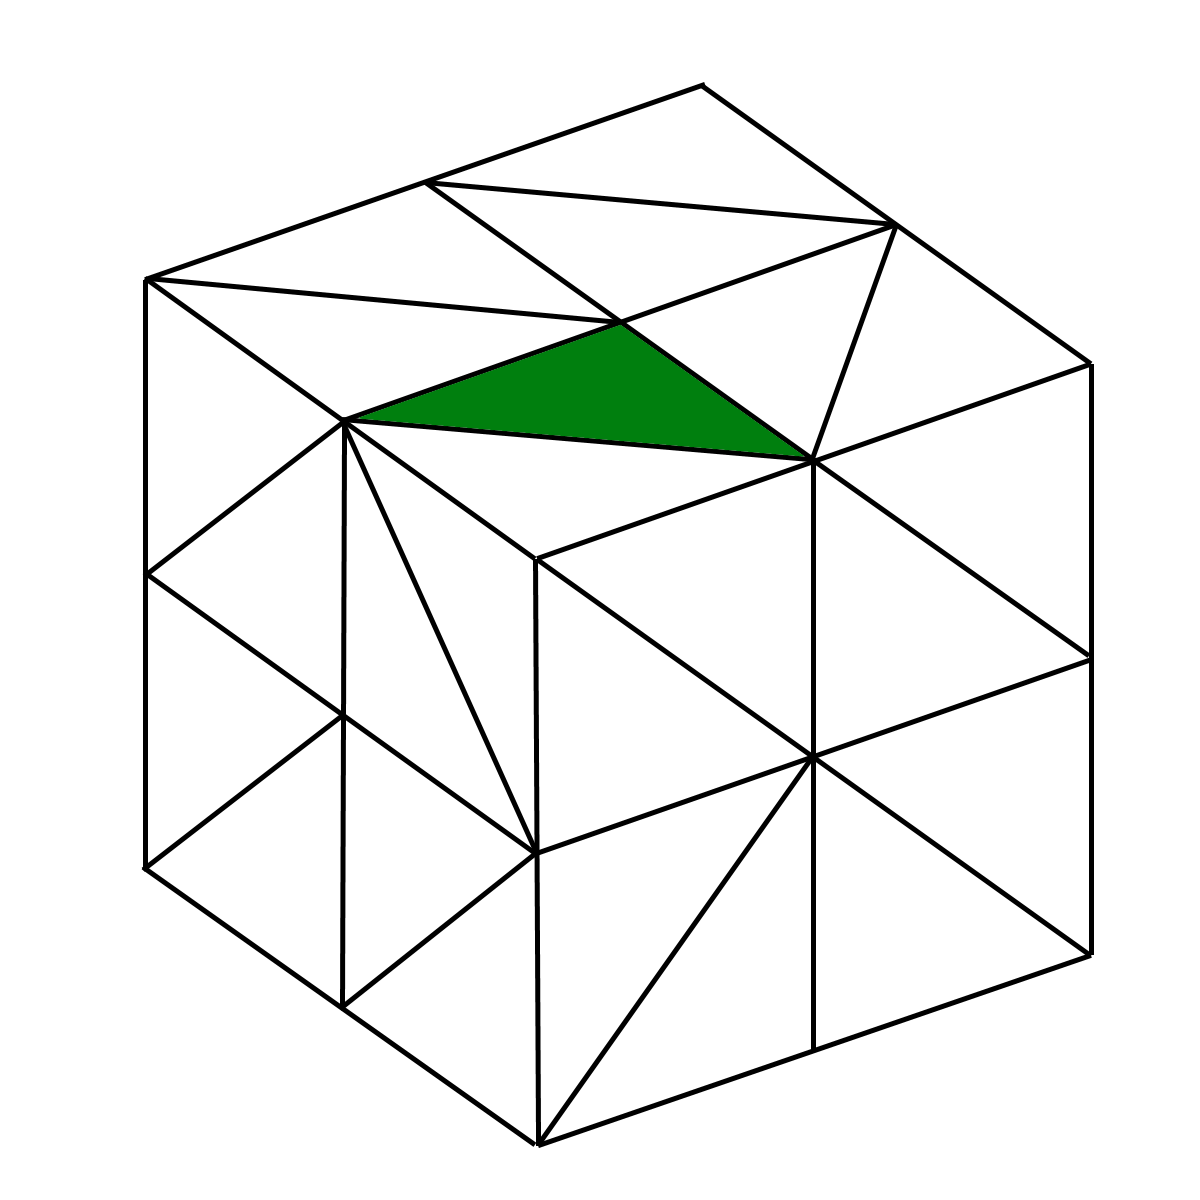
\includegraphics[width=\textwidth]{coplanar_algorithm_1.png}
    \caption{An arbitrary face is selected as starting face (marked green).}
    \label{fig:coplanar_algorithm_1}
  \end{subfigure}
  \begin{subfigure}[t]{0.4\textwidth}
    \centering
    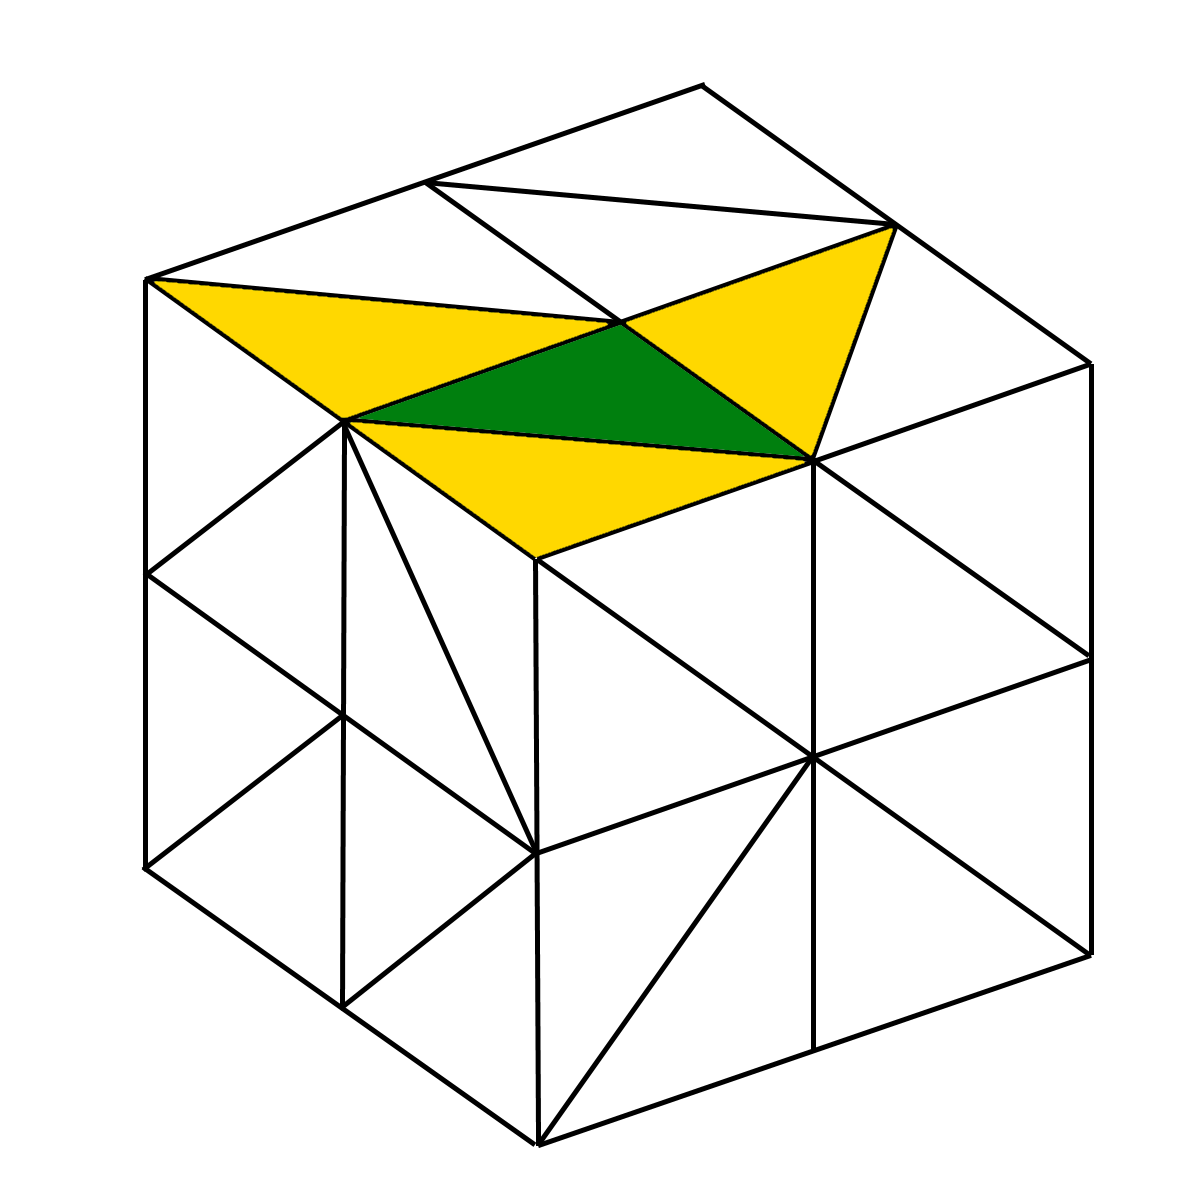
\includegraphics[width=\textwidth]{coplanar_algorithm_2.png}
    \caption{The adjacent faces are checked for coplanarity (marked yellow).}
    \label{fig:coplanar_algorithm_2}
  \end{subfigure}
  \begin{subfigure}[t]{0.4\textwidth}
    \centering
    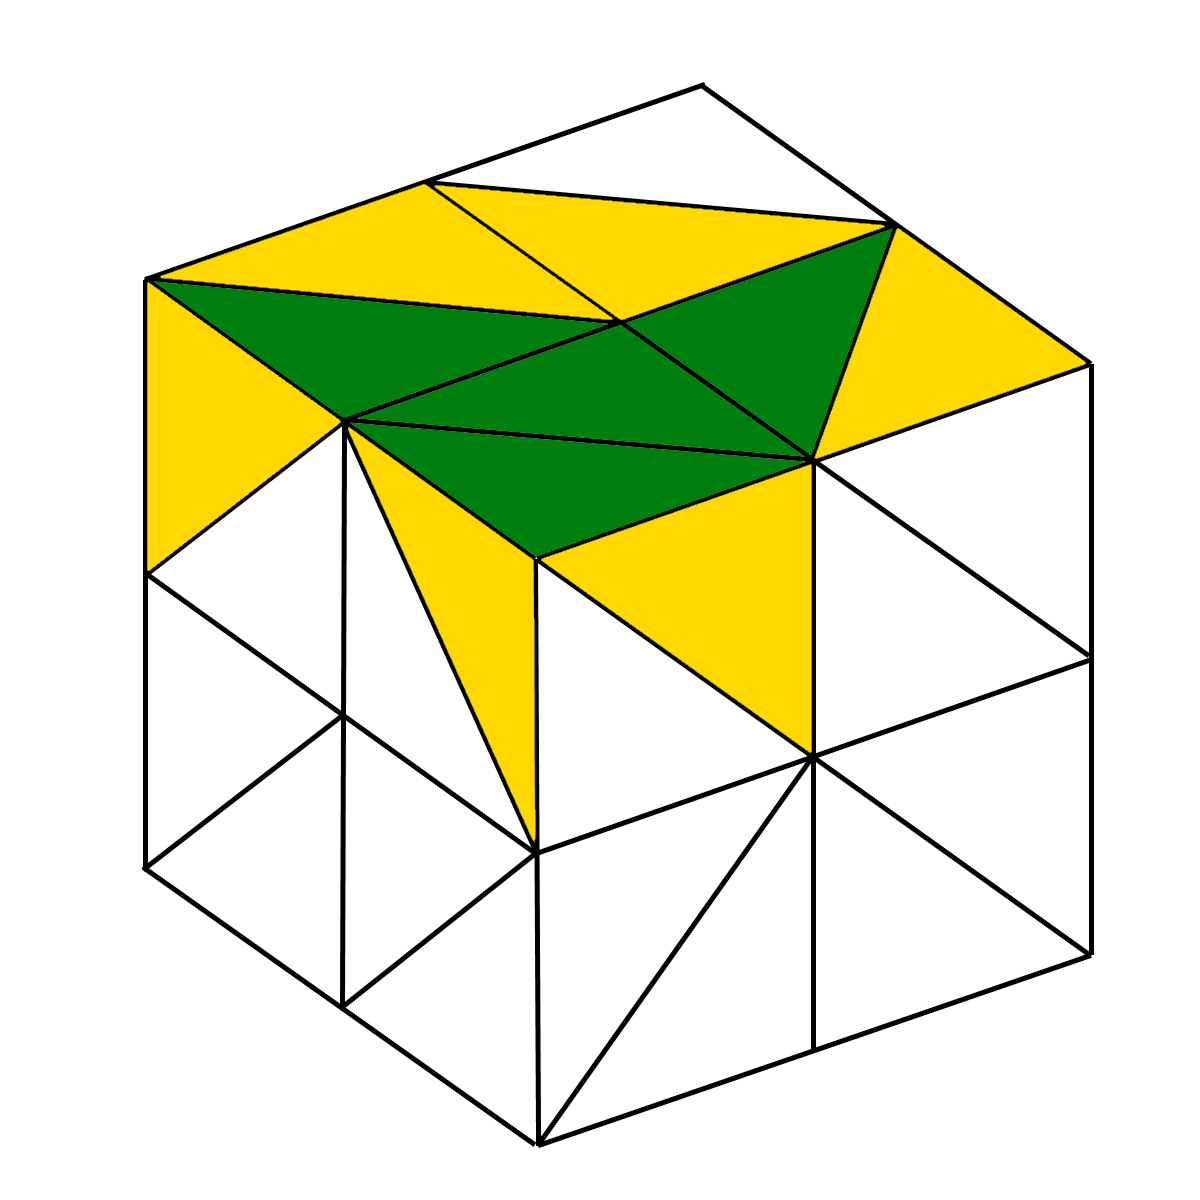
\includegraphics[width=\textwidth]{coplanar_algorithm_3.png}
    \caption{Since they are coplanar, the faces are added to the group. Now, their adjacent faces are tested.}
    \label{fig:coplanar_algorithm_3}
  \end{subfigure}
  \begin{subfigure}[t]{0.4\textwidth}
    \centering
    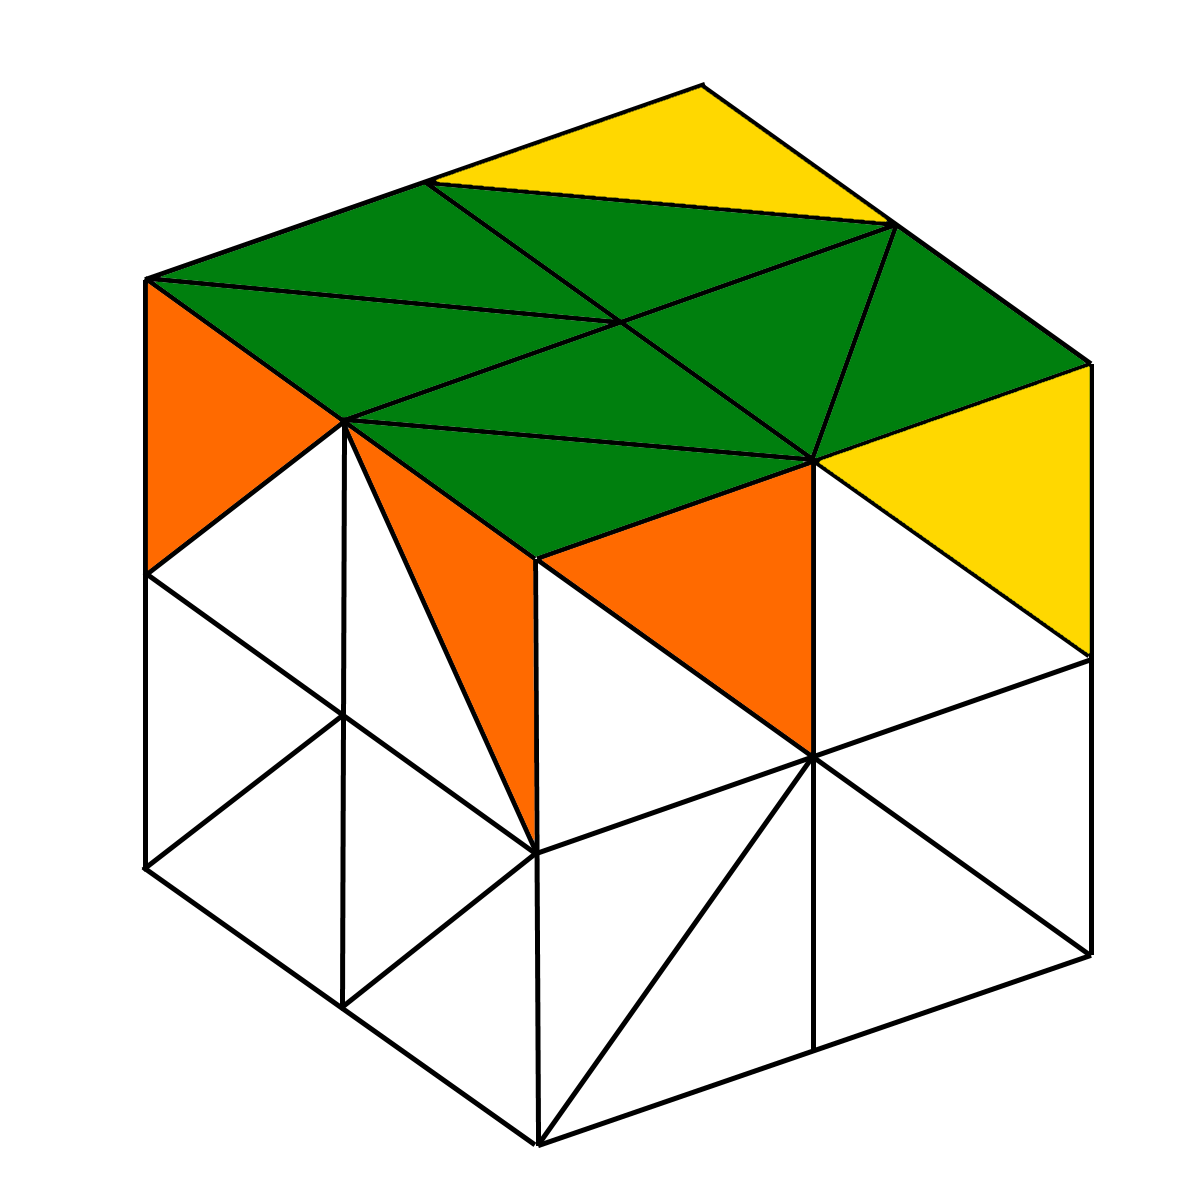
\includegraphics[width=\textwidth]{coplanar_algorithm_4.png}
    \caption{The coplanar faces are added to the group (green). The orange faces fail the coplanarity check and thus are not added.}
    \label{fig:coplanar_algorithm_4}
  \end{subfigure}
  \caption{\emph{CoplanarFaces} algorithm illustrated.}
  \label{fig:coplanar_algorithm}
\end{figure}

After all faces have been processed and assigned a group, the \mintinline{coffeescript}{faceGroups}, \mintinline{coffeescript}{faceGroupNormals} and \mintinline{coffeescript}{outerEdgeGroups} are injected into the face-vertex mesh, along with the \mintinline{coffeescript}{faceToFaceGroup} lookup table.

\subsection{Shape Finder}\label{sub:shapesfinder}

The shape finder creates shapes from the outer edge loops of the found coplanar faces. The outer edge loop is a set of edges in the format [vertex\_index\_1, vertex\_index\_2]. This is converted into a set of continuous edge loops of the form [vertex\_index\_1, vertex\_index\_2, ..., vertex\_index\_n, vertex\_index\_1].

To do so the \emph{mergeEdges} function is called until no edge segments can be merged anymore (see Listing~\ref{lst:mergeEdges}). This try to merge two edge segments which is possible if the starting or ending point of one of them matches the starting or ending point of the other (see Listing~\ref{lst:mergeEdgeStrings}).

The resulting sets of continues edge loops are converted into \class{shapes} (see Listing~\ref{lst:createShape}). Therefore from each edge loop the last vertex is removed because it is the same as the first and our \class{edgeLoops} do not need this redundancy. Afterwards all vertex indices are mapped to there corresponding coordinated because we thus for our further calculations. This vertex sets are used to create \class{edgeLoops}.

With the resulting \class{edgeLoops} we try to create a \class{shape}. \note{TO DO: explain InvalidNormalError?}

\note{TO DO: figures?}

\begin{listing}
\begin{minted}[
linenos,breaklines
]{coffeescript}
mergeEdges: (inEdges, same) ->
  # take first edgeloop
  edges = [inEdges.shift()]

  # try to merge into other edgeloop
  merged = no
  for inEdge in inEdges
    added = no
    for edge, i in edges when not added
      newEdge = @mergeEdgeStrings edge, inEdge, same
      if newEdge
        added = yes
        edges[i] = newEdge
    if not added
      edges.push inEdge
    else
      merged = yes
  return { edges, merged }
\end{minted}
\caption{Merging edge segments to continuous edge loops.}
\label{lst:mergeEdges}
\end{listing}

\begin{listing}
\begin{minted}[
linenos,breaklines
]{coffeescript}
mergeEdgeStrings: (
  edgeString,
  otherEdgeString,
  comparator = identityComparator
  ) ->
  lastIndex = edgeString.length - 1
  otherLastIndex = otherEdgeString.length - 1

  if comparator(edgeString[0], otherEdgeString[otherLastIndex])
    return otherEdgeString.concat(edgeString.slice(1))

  if comparator(otherEdgeString[0], edgeString[lastIndex])
    return edgeString.concat(otherEdgeString.slice(1))

  if comparator(edgeString[0], otherEdgeString[0])
    return edgeString.slice().reverse().concat(otherEdgeString.slice(1))

  if comparator(edgeString[lastIndex], otherEdgeString[otherLastIndex])
    return otherEdgeString.concat(edgeString.slice(0, -1).reverse())

  return null
\end{minted}
\caption{Merging edge segments to continuous edge loops.}
\label{lst:mergeEdgeStrings}
\end{listing}

\begin{listing}
\begin{minted}[
linenos,breaklines
]{coffeescript}
createShape: (shape, groupIndex, faceVertexMesh) ->
  newEdgeLoops = []
  for _edgeLoop in shape
    edgeLoop = _edgeLoop.slice()
    edgeLoop.pop()

    for vertex, vertexIndex in edgeLoop
      vertex *= 3
      edgeLoop[vertexIndex] = new THREE.Vector3(
        faceVertexMesh.vertexCoordinates[vertex]
        faceVertexMesh.vertexCoordinates[vertex + 1]
        faceVertexMesh.vertexCoordinates[vertex + 2]
      )

    newEdgeLoop = new EdgeLoop(edgeLoop)
    newEdgeLoops.push newEdgeLoop

  try
    shape = new Shape(
      newEdgeLoops,
      faceVertexMesh.faceGroupNormals[groupIndex],
      faceVertexMesh,
      groupIndex
    )
  catch error
    if error.name is "InvalidNormalError"
      shape = new Shape(newEdgeLoops, new THREE.Vector3(0, 0, 1))
      shape.isCorrupted = true
    else throw error
  { removalCount, shouldBeDeleted } =
   PointOnLineRemover.removeUnnecessaryVerticesInShape shape
  @_removedVerticesCount += removalCount
  if shouldBeDeleted
   return null
  return shape
\end{minted}
\caption{Creating a \class{shape} out of a set of continuous edge loops.}
\label{lst:createShape}
\end{listing}



\subsection{Hole Detection}\label{sub:holedetection}

The pipeline step \emph{HoleDetection} is run after \emph{ShapesFinder} and categorises every \emph{edgeLoop} of each \emph{shape} either as outer contour or as hole. This is done by computing their areas and comparing them: The \emph{edgeLoop} with the biggest area is the outer contour and all others are holes.



\section{Inherent Plates Require Parallel Top and a Bottom Shapes}\label{sec:inherentplates}

In order to find inherent plates in a mesh, all pairs of shapes have to be tested. The shapes have to be parallel to each other. Additionally, the distance between them is checked. In must fit one of the given plate thicknesses.

\subsection{Parallelism Is Checked Using Vector Functions}

The parallelism check uses vector functionality provided by \threejs{}. After ensuring that the normals are parallel, we have to test if they are facing apart. Without this requirement, holes in objects could be recognized as plate. An example is shown in Figure~\ref{fig:inherent_faceapart}. The vectors A and B in Figure~\ref{fig:inherent_faceapart:no} are facing towards each other. Using a vertex of vector A's shape and a vertex of vector B's shape, a new vector C is created. Since the angle between vector B and C is bigger than 90\textdegree{}, the shaped must face towards each other. Figure~\ref{fig:inherent_faceapart:yes} shows a valid example: The angle between vector B and C is smaller than 90{\textdegree}, thus the shapes are facing apart. In this case, a plate can be created.

\begin{figure}
  \centering
  \begin{subfigure}[t]{0.49\textwidth}
    \centering
    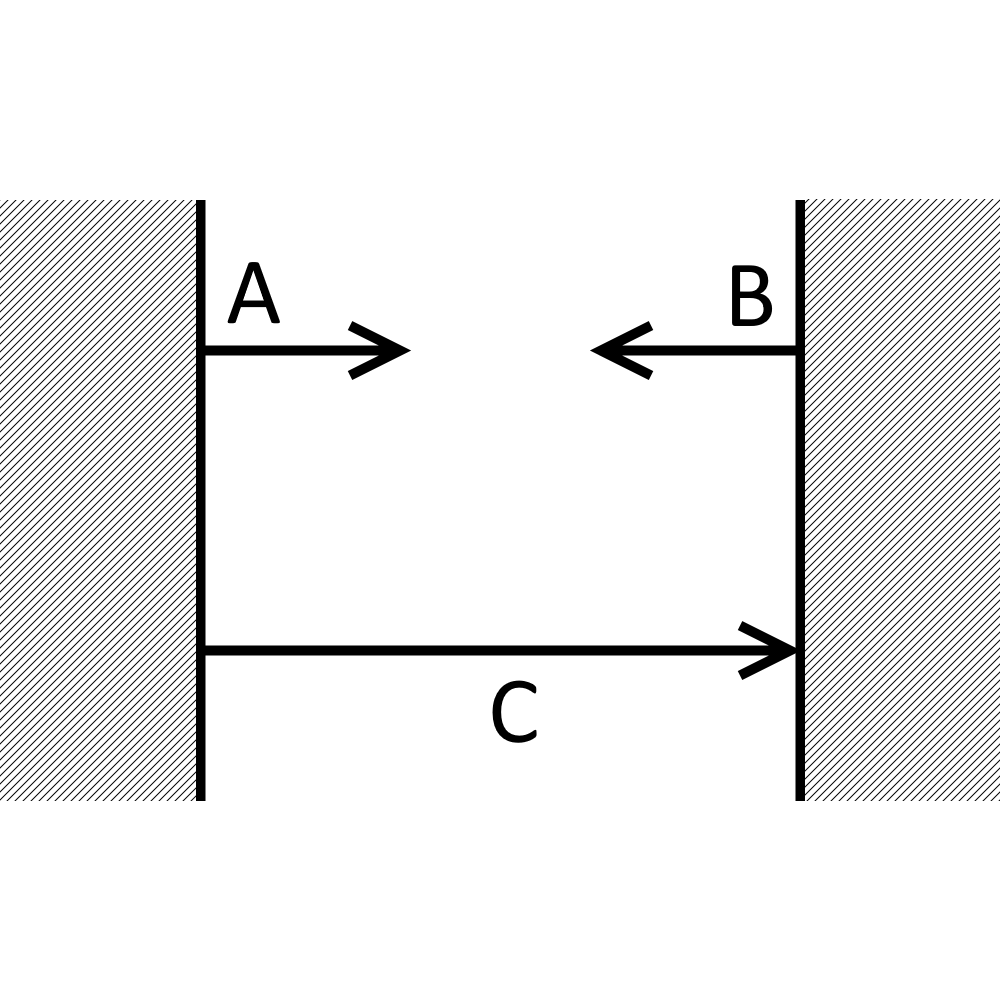
\includegraphics[width=0.7\textwidth]{inherent_faceapart_no.png}
    \caption{The normals are facing towards each other. No plate should be created.}
    \label{fig:inherent_faceapart:no}
  \end{subfigure}
  \begin{subfigure}[t]{0.49\textwidth}
    \centering
    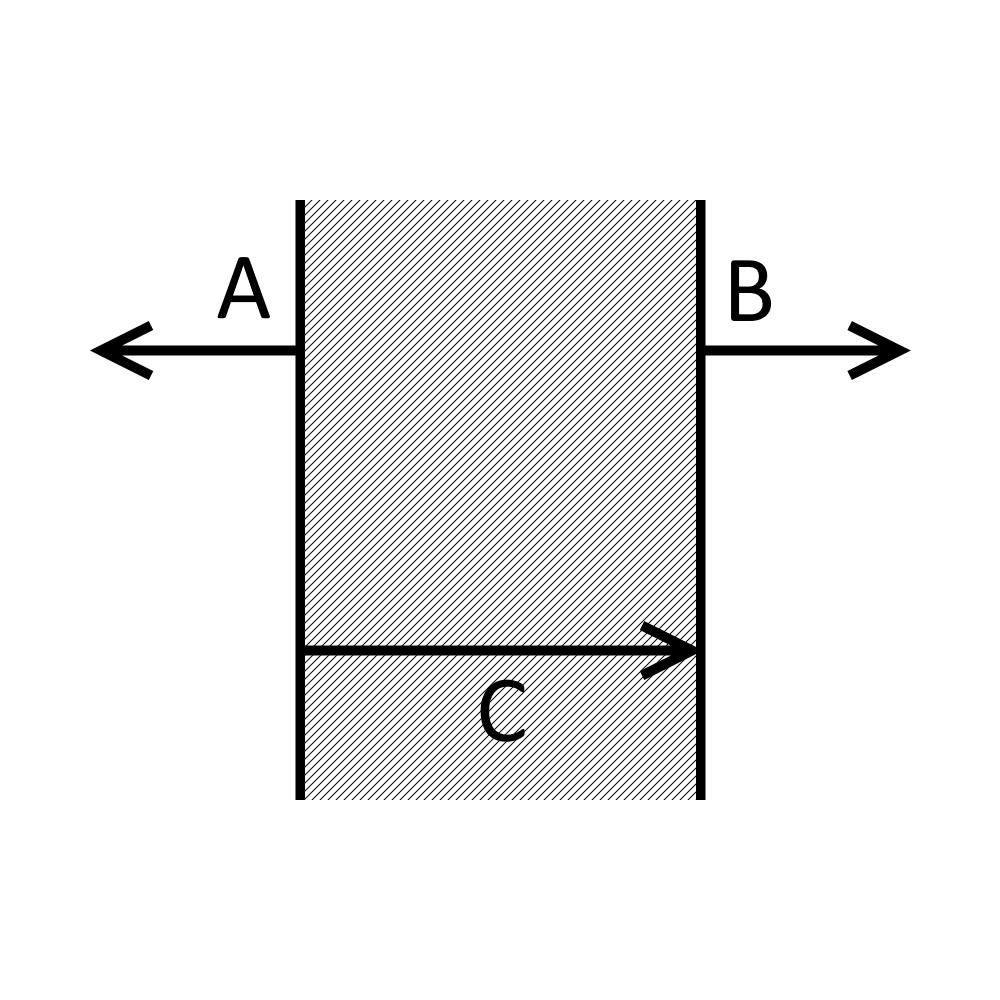
\includegraphics[width=0.7\textwidth]{inherent_faceapart_yes.png}
    \caption{The normals are facing apart. The test is successful.}
    \label{fig:inherent_faceapart:yes}
  \end{subfigure}
  \caption{Checking if the shapes' normals are facing apart avoids creating unwanted plates.}
  \label{fig:inherent_faceapart}
\end{figure}

\subsection{Calculating the Best Plate Thickness}

The calculation of the optimal plate thickness is shown in Listing~\ref{lst:checkplatethickness}. First, the actual distance between the shapes is calculated. Next, all possible plate thicknesses are tested if they can approximate the actual thickness well enough. Lastly, the thickness with the lowest absolute deviation is chosen as the best thickness. Since the user selects which materials he has available, only those can be used. Thus, we do not use the actual thickness for our calculations, but rather the chosen best thickness.

\begin{listing}
\begin{minted}[
linenos,breaklines
]{coffeescript}
checkPlateThickness: (shape1, shape2) ->
  actualThickness = @distanceBetweenPlanes shape1, shape2
  okThicknesses = []
  # check which thicknesses are ok factor-wise
  for plateThickness in @plateThicknesses
    if plateThickness * @minThicknessDeviationFactor < actualThickness < plateThickness * @maxThicknessDeviationFactor
      okThicknesses.push plateThickness
  bestThickness = null
  bestDeviation = null
  for plateThickness in okThicknesses
    deviation = Math.abs(plateThickness - actualThickness)
    if bestDeviation is null or deviation < bestDeviation
      bestDeviation = deviation
      bestThickness = plateThickness
  return bestThickness
\end{minted}
\caption{Finding the best plate thickness.}
\label{lst:checkplatethickness}
\end{listing}

\subsection{Creating Plates}

The plate creation uses the shapes' 2D representation, which is calculated when creating the shape. The vertices are rotated around the origin so that they have the same x-value. We use the shape's normal to build a rotation matrix, which is applied to a clone of each vertex. This rotation matrix is stored in the shape, while each of the shape's \emph{edgeLoops} contains the corresponding rotated vertices. Since the rotation is performed deterministically, we can use the 2D representation to perform operations like inctersection and union on shapes.

After finding these plate candidates, the shape which plane's distance to the origin (the z-value of all vertices when laid into the x-y-plane) is smaller is selected as the base shape of the plate, as shown in Listing~\ref{lst:faceintersect}. We only use one shape to represent the plate, since both shapes have to be congruent anyway. The other shape can be restored by translating the base shape using its normal and the plate's thickness. Now, the intersection of both shapes is calculated. This is done by using the 2D representation. The resulting intersection is transformed back into 3D space using the rotation matrix of the base shape. With the resulting shape, the plate is created.

\begin{listing}
\begin{minted}[
linenos
]{coffeescript}
shape2CloserToOrigin = abs(shape2.zValue) < abs(shape1.zValue)
polygon1 = create2DPolygon(shape1)
polygon2 = create2DPolygon(shape2)
intersection = polygon1.intersect polygon2
shapes = parseToShapes(intersection)
plates = parseToPlates(shapes)
return plates
\end{minted}
\caption{Face intersection for creating inherent plates.}
\label{lst:faceintersect}
\end{listing}

The intersection between the shapes is done using a customized branch\footnote{\url{https://github.com/platener/jsclipper}} of the {\jsclipper} library, which adds floating poing coordinates support, as well as automatic data type conversion. After parsing them into the library's polygon class (see Section~\sectionref{sec:datasructures}), they can be easily clipped, resulting in a list of intersections which can be parsed back into shapes. To obtain the vertices in 3D space, we use the previously calculated rotation matrix. The plate creation is based on the previously selected base shape. While the calculated intersection is used as the shape of the plate, the thickness is computed by subtracting the base shape's z-value from the other shape's z-value. Additionally, the base shape's z-value is used as plane constant.

\section{Extruding Plates}\label{sec:extrudedplates}

The extrusion of plates is a simpler approach in terms of calculation, which is shown in Listing~\ref{lst:extrude}. The selected plate thickness has to be inverted, due to the plate being extruded in the opposite direction of the face's normal. The plane constant of the plates base plane is the same as the z-value of the shapes x-y-representation. We compare the face's area to a threshold, which filters plates which would be to small to fabricate. Afterwards, the new plate is created.

\begin{listing}
\begin{minted}[
linenos
]{coffeescript}
createPlateFromShape: (shape) ->
  thickness = -@plateThicknesses[0]
  planeConstant = shape.edgeLoops[0].xyPlaneVertices[0].z
  if shape.getContour().computeArea() > @areaThreshold
    return new Plate shape, thickness, planeConstant
  else
    return null
\end{minted}
\caption{Extruding a plate from a shape.}
\label{lst:extrude}
\end{listing}

\section{Removing Contained Plates}\label{sec:removingContainedPlates}

\emph{RemoveContainedPlates} is executed after plate generation and removes unnecessary ones that appear with our software.

There are two types of plates that get deleted: First as already described in the master thesis \emph{Platener} \cite{master-thesis} in Section '4.4.4 Removing contained plates', small plates can be created that completely lie inside another plate. Second there may be parallel plates that lie inside each other. That occurs due to extrusion if the the 3D object is modeled with thicker blocks than the available material thickness.

We iterate over all plates and compare them to all other plates. The comparison is based on their normals while further checks are not necessary most of the time because the normal check excludes most of them. Therefore the comparison is fast enough and the amount of comparisons must not be reduced with a different iteration algorithm.

\subsection{Plate Contains Other Plate Completely}

As described in the master thesis the algorithm may produce small plates that lie completely inside the actual modeled plate. These plates are orthogonal.

So if two plates have orthogonal normals we check if one of them lies completely in the other and remove it.


\subsection{Overlapping Parallel Plates}

A 3D block can not be represented by one single plate if it is thicker than a plate. The software creates two plates instead. The resulting plates will overlap in case this block is thinner than those two plates together.

So if two plates are parallel we compare their plane constants which specify the distance to the origin. In case the plane constants hint at overlap the actual \emph{EdgeLoops} are compared to identify intersections. In case they overlap one of the plates gets deleted.


\section{Stacking Plates}\label{sec:stackedplates}

As an alternative approach, plates can be stacked. An example is shown in Figure~\ref{fig:stackedbunny}. By putting multiple plates on top of each other, the model is approximated. In order to achieve this, the model is sliced in regular intervals, with plates being created based on the cross sections. In order to enable easy assembly, the plates are connected with shafts. These are additional plates, which are perpendicular to the other plates and help to align them.

\begin{figure}
    \centering
    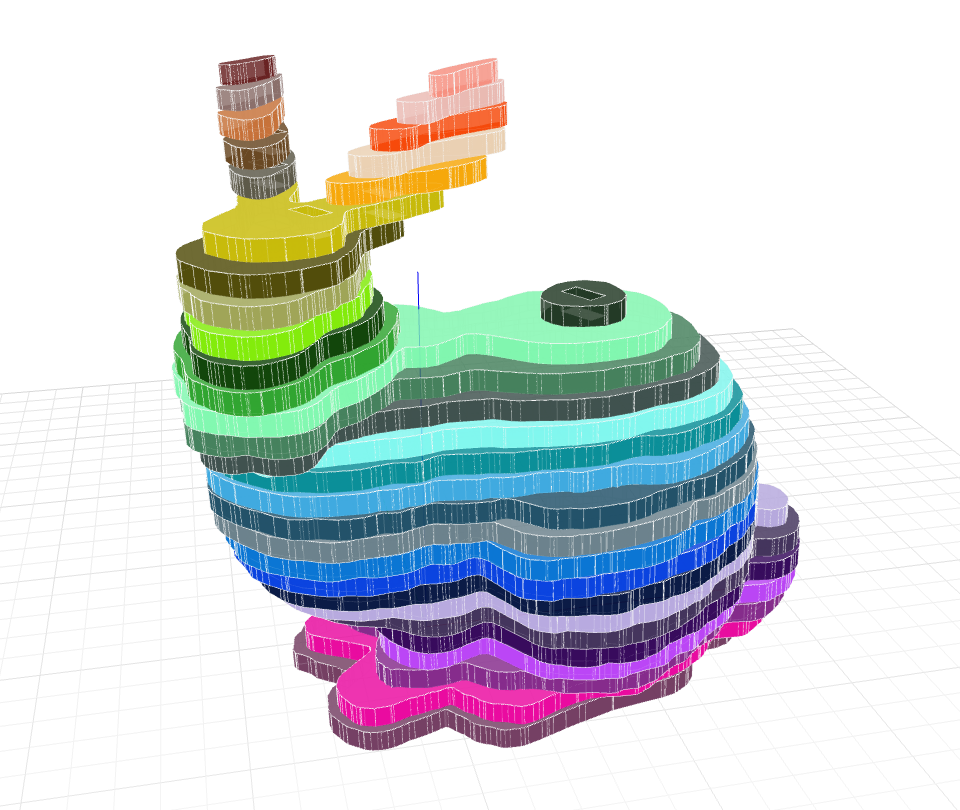
\includegraphics[width=.5\textwidth]{Images/bunny_1.png}
    \caption{Stacked plates can be used to approximate the model.}
    \label{fig:stackedbunny}
\end{figure}

The main function for stacking is shown in Listing~\ref{lst:stackedmain}. First, the model is rotated in order to optimize the stacking direction. Afterwards, the clipping planes are calculated. These plates are parallel to the x-y-plane. They are used to create cross-sections of the model. This is done by intersecting each of the model's faces with these plates. Afterwards, the resulting edges are merged into edge loops, which are used for creating shapes and, as helper objects, polygons. With these, shafts can be added, which connect plates for easier assembly. Afterwards, plates are created. These have to be rotated back based on the original rotation in order to align them with the model. 

\begin{listing}
\begin{minted}[
linenos
]{coffeescript}
findStackedPlates: (model, shapes) ->
  return new Promise (resolve) =>
    rotationMatrix = @findRotation shapes
    model.getClone().then((clone) =>
      @model = @rotateModel clone, rotationMatrix
      @planes = @getClippingPlanes()
      @clipFacesAgainstPlanes @model.model.mesh.faces
      @mergeEdgesInPlanes()
      @shapeGroups = @createShapes()
      @polygonGroups = @createPolygons()
      @shafts = @findShafts()
      @shapes = @clipShafts()
      plates = @createPlates().filter((p) -> p?)
      shaftPlates = @createShaftPlates()
      plates = plates.concat shaftPlates
      plates = @rotatePlatesBack plates, rotationMatrix
      resolve plates
    )
\end{minted}
\caption{Plate stacking main function.}
\label{lst:stackedmain}
\end{listing}

\subsection{Rotating the Model}

In order to find a good rotation, the model's biggest surface is aligned to the x-y-plane. A good rotation results in fewer plates which are preferably all connected. Figure~\ref{fig:stackingorientations} shows how different rotations yield in different results. While the approach of stacking plates doesn't require information about the model's coplanar surfaces, this optimization does. By iteration over them, the biggest surface's rotation matrix can be found (see Listing~\ref{lst:findrotation}). This matrix can be used for transforming all vertices so that the chosen surface is parallel to the x-y-plane.

\begin{figure}
  \centering
  \begin{subfigure}[t]{0.4\textwidth}
    \centering
    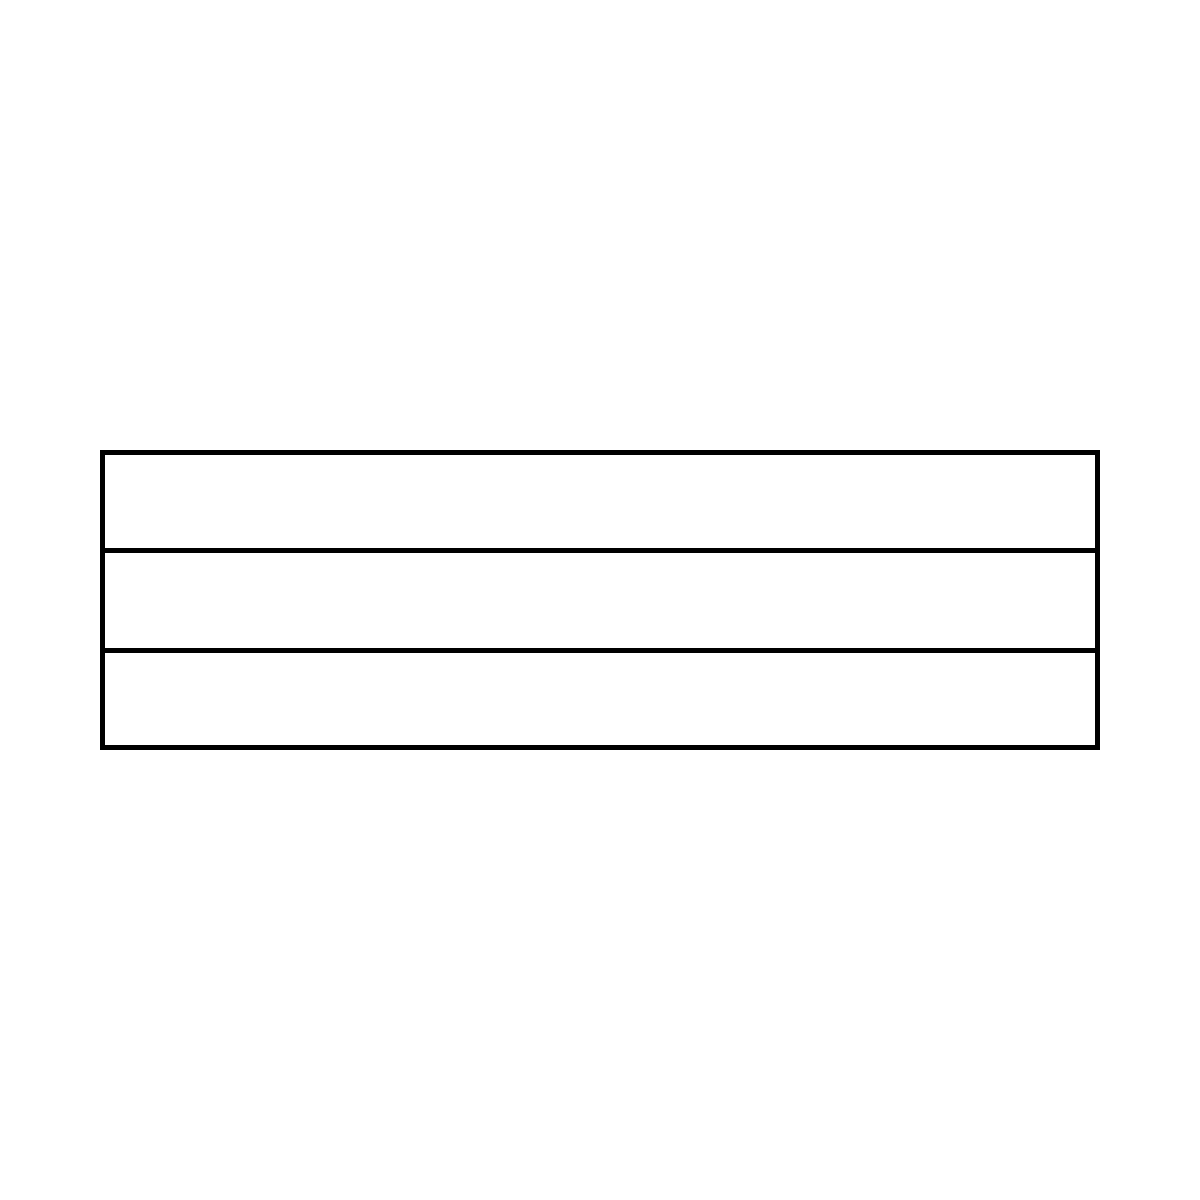
\includegraphics[width=\textwidth]{stacked_orientation_good.png}
  \end{subfigure}
  \begin{subfigure}[t]{0.4\textwidth}
    \centering
    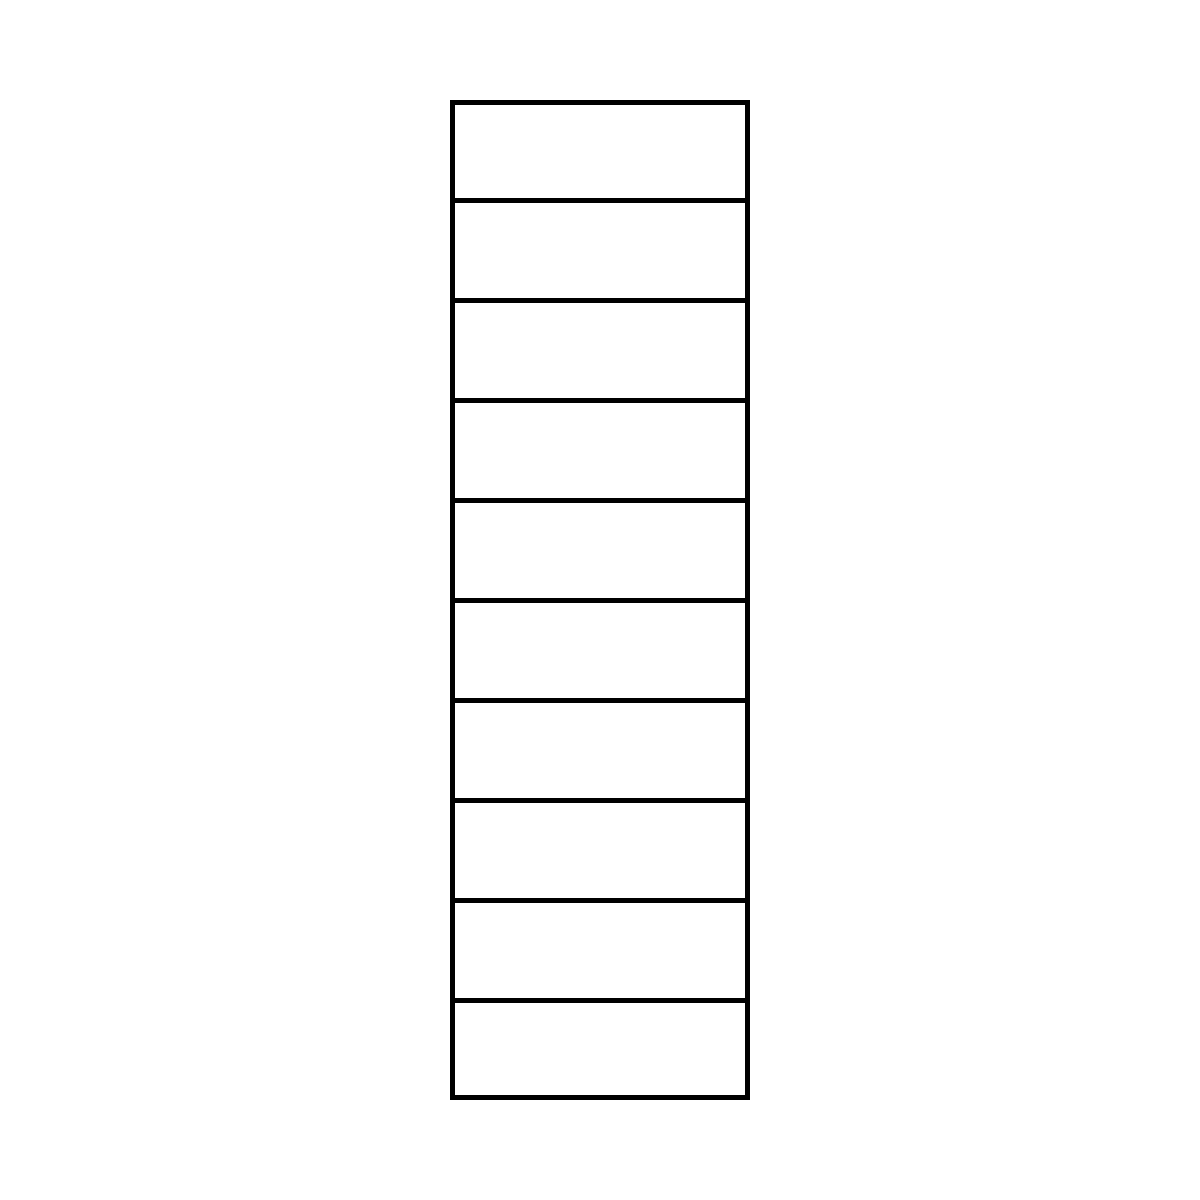
\includegraphics[width=\textwidth]{stacked_orientation_bad.png}
  \end{subfigure}
  \caption{Different stacking directions yield different results.}
  \label{fig:stackingorientations}
\end{figure}

\begin{listing}
\begin{minted}[
linenos
]{coffeescript}
findRotation: (shapes) ->
  maxArea = 0
  rotationMatrix = new THREE.Matrix3()
  shapes.forEach((shape) ->
    area = shape.area || shape.getContour().computeArea()
    if area > maxArea
      maxArea = area
      rotationMatrix = shape.rotationMatrix
  )
  return rotationMatrix
\end{minted}
\caption{Finding an optimal rotation.}
\label{lst:findrotation}
\end{listing}

\subsection{Finding the Clipping Planes}

Due to the model being rotated, it can be sliced using planes parallel to the x-y-plane. In order to calculate these, the model's bounding box is calculated first. Using the minimal and maximal z-value, planes are creates with an distance equal to the selected plate thickness. These planes are constructed from a {\threejs} plane object and a (initially empty) list of edges located in this plane. The planes are displaced by half the plate thickness. Thus, the sampling happens in the middle of the plates, which is an approximation which works for most applications. The plane creation is shown in Listing~\ref{lst:clippingplanes}.

\begin{listing}
\begin{minted}[
linenos,breaklines
]{coffeescript}
getClippingPlanes: ->
  planes = []
  for i in [@minZ..@maxZ] by @thickness
    planes.push {
      plane: new THREE.Plane(
        new THREE.Vector3(0, 0, 1), 
        -(i + @thickness / 2)
      )
      edges: []
    }
  return planes
\end{minted}
\caption{Clipping plane generation.}
\label{lst:clippingplanes}
\end{listing}

\subsection{Intersecting the Model's Faces with the Clipping Planes}

Clipping each face with each plane would be very slow. Thus, we first find one plane which clips the face and check the adjacent planes afterwards (see Listing~\ref{lst:clipfaceplanes}). I order to quickly find this plane, binary search is used, as shown in Listing~\ref{lst:findplane}. Starting at the median plane (\mintinline{coffeescript}{@planes.length // 2}), we search the planes until one plane clipping the face is found or it is certain that no plane clips the face.

\begin{listing}
\begin{minted}[
linenos
]{coffeescript}
clipFaceAgainstPlanes: (face) ->
  planeIndex = @findClippingPlane(face)
  if planeIndex > -1
    @checkAdjacentPlanes(face, planeIndex)
\end{minted}
\caption{Clipping a face against all planes.}
\label{lst:clipfaceplanes}
\end{listing}

\begin{listing}
\begin{minted}[
linenos,breaklines
]{coffeescript}
findClippingPlane: (face) ->
  stepWidth = @planes.length / 4.0
  index = -1
  currentIndex = @planes.length // 2
  oldIndex = -1
  while currentIndex isnt oldIndex and 0 <= currentIndex < @planes.length and index is -1
    direction = @clipFaceAgainstPlane(
      face, 
      @planes[currentIndex]
    )
    # found clipping plane
    if direction is 0
      index = currentIndex
    # continue search
    else
      oldIndex = currentIndex
      currentIndex += Math.round stepWidth * direction
      stepWidth /= 2
  return index
\end{minted}
\caption{Finding a plane which clips the face.}
\label{lst:findplane}
\end{listing}

The search direction is calculated by clipping the face against the plane (Listing~\ref{lst:clipfaceplane}). After clipping each edge with the face, the number of intersection decides the result.

\begin{itemize}
  \item No intersections: The face does not clip the plane.
  \item One Intersection: Invalid. It is not possible to get only one intersection when clipping a valid face.
  \item Two intersections: If both intersection points are the same, one vertex of the face clips the plane. Otherwise two edges clip the plane.
  \item Three intersections: If any two of the intersection points are the same, a vertex and the opposite edge clip the plane. Otherwise the whole face lies in the plane.
\end{itemize}

If the face does not clip the plane or only intersect with one vertex, we check if it is below or above the plane and return either -1 or 1 as direction (calculation shown in Listing~\ref{lst:facedirection}). In all other cases, 0 is returned, because the face clips the plane and we don't have to search further. 

Additionally, if either two edges, an edge and a vertex or the whole face clips the plane, these intersections are stored in the plane.

\begin{listing}
\begin{minted}[
linenos
]{coffeescript}
clipFaceAgainstPlane: (face, plane) ->
  intersections = []
  face.vertices.forEach((vertex, index) =>
    start = vector(vertex)
    end = vector(face.vertices[(index + 1) % 3])
    line = new THREE.Line3(start, end)
    intersection = plane.plane.intersectLine line
    if intersection? then intersections.push intersection
  )
  # handle intersections
  # [...]
  return direction
\end{minted}
\caption{Clipping a face against a plane.}
\label{lst:clipfaceplane}
\end{listing}

\begin{listing}
\begin{minted}[
linenos
]{coffeescript}
getDirectionFromPlaneToFace: (face, plane) ->
  sum = 0
  face.vertices.forEach((vertex) ->
    sum += vertex.z + plane.plane.constant
  )
  if sum is 0 then throw new Exception()
  return sum / Math.abs sum
\end{minted}
\caption{Calculating the direction from a plane to a face.}
\label{lst:facedirection}
\end{listing}

After one plane which intersect the face has been found, the adjacent ones have to be checked as well, since a face can span over multiple planes. This is done by iterating over the planes, starting from the next one and moving away. If the returned direction is not 0, we can stop because the plane and all following ones do not clip the face. Both directions, upwards and downwards, are checked separately (see Listing~\ref{lst:checkadjacent}).

\begin{listing}
\begin{minted}[
linenos,breaklines
]{coffeescript}
checkAdjacentPlanes: (face, index) ->
  runIndex = index + 1
  direction = 0
  while(runIndex < @planes.length and direction is 0)
    direction = @clipFaceAgainstPlane(
      face, 
      @planes[runIndex++]
    )
  runIndex = index - 1
  direction = 0
  while(runIndex >= 0 and direction is 0)
    direction = @clipFaceAgainstPlane(
      face, 
      @planes[runIndex--]
    )
  return
\end{minted}
\caption{Checking if adjacent planes are clipping too.}
\label{lst:checkadjacent}
\end{listing}

\subsection{Creating Shapes/ Mehr Umschreibender Title}

Using the intersections stored in each plane, shapes can be created. This is done using the \emph{ShapesFinder}, which is described in Section~\sectionref{sub:shapesfinder}. Instead of the outer edges of face groups (see Section~\sectionref{sub:coplanarfaces}), the intersections between the faces and the clipping planes are used. The resulting shapes represent the cross-sections of the model. Additionally, the {\jsclipper} library is used to create 2D polygons, which are used in the next step.

\subsection{Adding Shafts / Mehr Umschreibender Title}

In order to assemble the stacked plates, we connect them with shafts (Figure~\ref{fig:shafts}). Our approach for this: if two shapes which are located in adjacent planes intersect, they have to be connected by at least one shaft. The shaft finding algorithm has three steps: First, we iterate over all shapes and connect as many as possible. Next, we fix shapes which are not yet connected. Afterwards, we clean up shafts which are only connected to one shape. The shaft object contains a list of the polygon it connects, as well as the intersection of all these polygons.

\begin{figure}
    \centering
    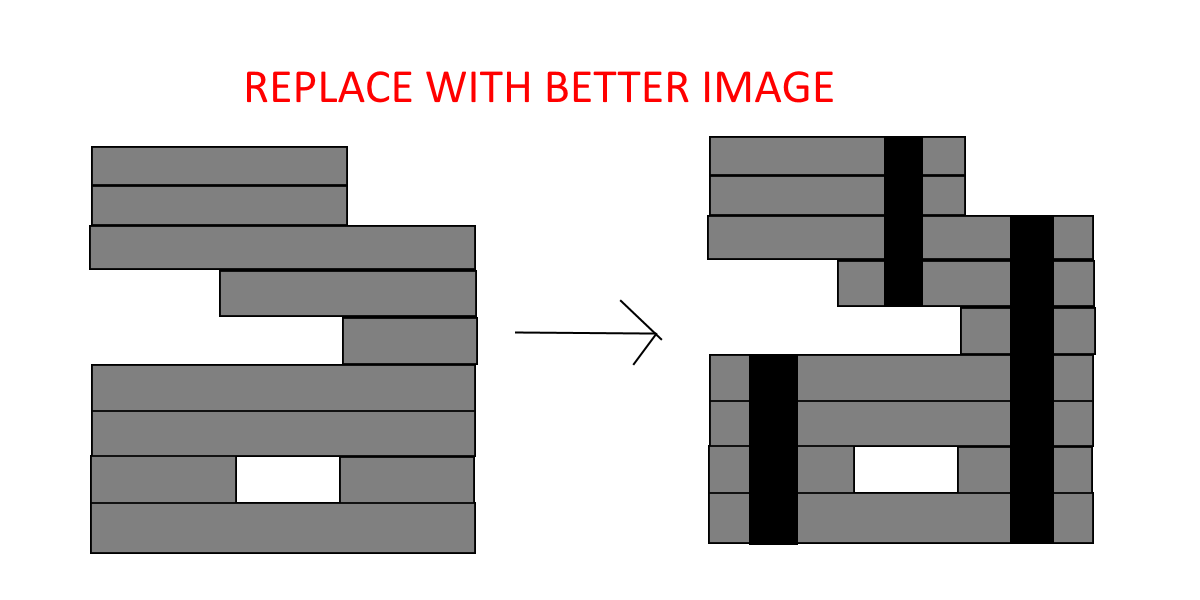
\includegraphics[width=1.0\columnwidth]{Images/plates_shafts.png}
    \caption{Connecting plates with shafts.}
    \label{fig:shafts}
\end{figure}

\subsubsection{First Pass / Mehr Umschreibender Title}

Instead of the actual shapes, the corresponding polygons are used, which enable working with the {\jsclipper}. These are organized in layers, matching the clipping planes. Each layer contains a list of polygons, since there can be multiple shapes in one layer. We have to iterate over both lists, the inner and the outer, as shown in Listing~\ref{lst:findshafts}.

When processing a new polygon, we first mark that it has not been added to any shaft yet. Now, we iterate over all shaft candidates. If the current level (the layer) is bigger than the shaft's last added polygon's level plus one, there was no polygon from the last layer added to the shaft. Since we do not want shafts to create "bridges" spanning between unconnected layers, the shaft is marked as completed. If that is not he case, we try to add the polygon to the shaft.

\begin{listing}
\begin{minted}[
linenos,breaklines
]{coffeescript}
findShafts: ->
  shaftCandidates = []
  @polygonGroups.forEach((polygonGroup, level) =>
    polygonGroup.forEach((polygon) =>
      added = false
      shaftCandidates.forEach((shaftCandidate) =>
        if level > shaftCandidate.lastlevel + 1
          shaftCandidate.finished = true
        if not shaftCandidate.finished
          if @tryAddingPolygonToShaftCandidate(
                polygon, shaftCandidate
              )
            shaftCandidate.lastlevel = level
            added = true
      )
      if not added
        if Shaft.isIntersectionBigEnoughForShaft(
              polygon.polygon, @shaftData
            )
          newShaftCandidate = Shaft.fromPolygon(
            polygon,
            level,
            @shaftData
          )
          newShaftCandidate.polygons[0].shafts.push(
            newShaftCandidate
          )
          @tryOverlappingShaftBackwards newShaftCandidate
          shaftCandidates.push newShaftCandidate
    )
  )
  @fixUnconnectedPlates shaftCandidates
  @cleanUpShafts shaftCandidates
  shaftCandidates.forEach((shaft) ->
    shaft.createShaftContourAndCrossSection()
  )
  return shaftCandidates
\end{minted}
\caption{Finding shafts.}
\label{lst:findshafts}
\end{listing}

Listing~\ref{lst:addpolytoshaft} shows the calculations run when adding a polygon to a shaft. First, the shaft's intersection and the new polygon are intersected. The resulting intersection is checked if it is big enough to fit the shaft. If that is the case, the shaft's intersection is updated and the polygon is added to the shaft.

\begin{listing}
\begin{minted}[
linenos,breaklines
]{coffeescript}
tryAddingPolygonToShaftCandidate: (
    polygon, shaftCandidate, direction
  ) ->
    clip = polygon.polygon.intersect shaftCandidate.intersection
    if clip.length > 0 and
        Shaft.isIntersectionBigEnoughForShaft clip[0], @shaftData
      newIntersection =
        new jsclipper.Polygon clip[0].getShape(), clip[0].getHoles()
      shaftCandidate.intersection = newIntersection
      if direction is "DOWN" then shaftCandidate.polygons.unshift polygon
      else shaftCandidate.polygons.push polygon
      polygon.shafts.push shaftCandidate
      return true
    return false # no intersection
\end{minted}
\caption{Adding a polygon to a shaft.}
\label{lst:addpolytoshaft}
\end{listing}

If the polygon can not be added to any of the shafts, we create a new one - if the polygon is big enough (Listing~\ref{lst:findshafts}). Additionally, the shaft is overlapped "backwards", up to three layers. This improves stability in the assembled model.

\subsubsection{Fixing unconnected plates}

In some cases, not all polygons - and thus not all plates - are connected to the others yet. Additionally, shafts should be expanded in both directions as far as possible. A fix is shown in Listing~\ref{lst:fixunconnected}.

Each polygon is checked how well it is connected to other polygons. If it is connected to both a polygon below and above (\mintinline{coffeescript}{connection.isConnected} is true), we do not have to connect it further. Otherwise, the shafts connecting it from above and below are checked. We try to expand these to connect more polygons in the given direction. If this succeeds, handling for this polygon is completed. Otherwise, we create a new shaft at this polygon and try to expand it in both directions.

\begin{listing}
\begin{minted}[
linenos,breaklines
]{coffeescript}
fixUnconnectedPlates: (shaftCandidates) ->
  @polygonGroups.forEach((polygonGroup, level) =>
    polygonGroup.forEach((polygon) =>
      connection = @isPolygonConnected polygon, level
      if not connection.isConnected
        expanded = false
        direction = "DOWN"
        if connection.shaftsFromAbove.length > 0
        expanded = @tryExpandingShaftsInOneDirection(
          connection.shaftsFromAbove, level, direction
        )
        if connection.shaftsFromBelow.length > 0
          direction = "UP"
          expanded = @tryExpandingShaftsInOneDirection(
            connection.shaftsFromBelow, level, direction
          )
        if not expanded and 
            Shaft.isIntersectionBigEnoughForShaft(
              polygon.polygon, @shaftData
            )
          newShaftCandidate = Shaft.fromPolygon(
            polygon
            level
            @shaftData
          )
          newShaftCandidate.polygons[0].shafts.push(
            newShaftCandidate
          )
          @tryExpandingShaftAroundLevel(
            newShaftCandidate
            level
            direction
          )
          shaftCandidates.push newShaftCandidate
    )
  )
\end{minted}
\caption{Fixing unconnected plates.}
\label{lst:fixunconnected}
\end{listing}

\subsubsection{Cleaning up shafts / Mehr Umschreibender Title}

As a result of this method, polygons which are not adjacent to any other polygon get assigned an own shaft. Since this does not improve the models stability, these are removed again, as shown in Listing~\ref{lst:cleanupshafts}.

\begin{listing}
\begin{minted}[
linenos
]{coffeescript}
cleanUpShafts: (shafts) ->
  if shafts.length > 0
    for i in [shafts.length - 1..0]
      if shafts[i].polygons.length < 2
        shafts[i].polygons.forEach((polygon) ->
          polygon.shafts.splice polygon.shafts.indexOf(shafts[i]), 1
        )
        shafts.splice i, 1
\end{minted}
\caption{Cleaning up shafts.}
\label{lst:cleanupshafts}
\end{listing}

\subsection{Creating plates/ Mehr Umschreibender Title}

After the shafts are found, their cross section is cut from the connected polygons. Next, these polygons are parsed into shapes and plates. Additionally, the shafts' contours are calculated, with additional plates being created from them. Together, all plates are returned.

\end{document}